\documentclass{llncs}
\usepackage{graphicx}
\usepackage{color}
\usepackage{hyperref}
\hypersetup{
    colorlinks=true,
    linkcolor=blue,
    filecolor=magenta,      
    urlcolor=cyan,
}
%%%%%%%%%%%%%%%%%%%%%%%%%%%%%%%%%%%%%%%%%%%%%%%%%%%%%%%%%%%%%%%%%%%%%%%%%%
\usepackage{todonotes} % use this to see the comments
%\usepackage[textsize=tiny]{todonotes} % use this to see SMALL : ) comments
%\usepackage[disable]{todonotes} % use this to hide all comments
%%%%%%%%%%%%%%%%%%%%%%%%%%%%%%%%%%%%%%%%%%%%%%%%%%%%%%%%%%%%%%%%%%%%%%%%%%


\newcommand{\todoinline}[1]{
    \todo[inline]{#1}
}
\newcommand{\todoiteminline}[3]{
    \todoitemtemplate{#1}{#2}{#3}{inline}{red}
}

\newcommand{\todoproofread}[3]{
    \todoitemtemplate{#1}{#2}{Please proof read above section; #3}{inline}{yellow}
}
\definecolor{mygreen}{HTML}{00CC00}
\newcommand{\todoproofreadDone}[3]{
    \todoitemtemplate{#1}{#2}{Please proof reading above section, done; #3}{inline}{mygreen}
}
\newcommand{\todoproofreaddone}[3]{
    \todoproofreadDone{#1}{#2}{#3}
}

\newcommand{\todoitemtemplate}[5]{%
% \index[MYTODO]{#2}
\todo[#4,color=#5,caption=X]{{#1}{ \textbf{{\tiny{for}} #2}:}{#3}}%
}

\newcommand{\todoiteminlinedone}[3]{
    \todoiteminlineDone{#1}{#2}{#3}
}
\newcommand{\todoiteminlineDone}[3]{
    \todoitemtemplate{{\commentsDoneFont{#1}}}{{\commentsDoneFont{#2}}}{{\commentsDoneFont{#3}}}{inline}{green}
}

\newcommand{\todoitem}[3]{
    \todoitemtemplate{#1}{#2}{#3}{}{red}
}
\newcommand{\todoitemdone}[3]{
    \todoitemDone{#1}{#2}{#3}
}
\newcommand{\todoitemDone}[3]{{\commentsDoneFont\todoitemtemplate{{\commentsDoneFont{#1}}}{{\commentsDoneFont{#2}}}{{\commentsDoneFont{#3}}}{}{green}}}



\begin{document}


%\title{All about Indexing for Question Answering systems: A deep dive into Information retrieval}
%\title{Graph vs RDF stores: An Empirical Evaluation of NoSQL RDF Data Management Solutions}
%\title{An Empirical Evaluation of NoSQL RDF Data Management Solutions}
%\title{Benchmarking RDF Data Management Solutions}
\title{LITMUS: An open extensible benchmarking platform for NoSQL RDF Data Management Solutions}


\author{Harsh Thakkar, Mohnish Dubey, ... }

\institute{Enterprise Information Systems Lab, \\ University of Bonn, Germany \\ \vspace{10pt} \texttt{hthakkar@uni-bonn.de}}

\maketitle

\begin{abstract}

Abstract will appear here. \textit{When it's time!}

\end{abstract}

\section{Introduction}\label{sec:Introduction}
    \todoiteminline{Harsh}{co-authors}{This is pending}
    
    Introduction will appear here. your \framebox[1.0\width]{Box here} and text here. 
    
    {\color{green} outline:
    General introduction of current state of data and tool explosion\\
    Recent activity in this research area\\
    Our main contribution in this paper/work\\
    Outline of the paper.(Here we give all name of the section in the paper)\\ }
    
    The current era stands as a witness to the enormous explosion of structured data on the Web referred to as Linked Data\footnote{http://lod-cloud.net/}. With such a rapid growth in the amount of data, managing this data has also become a challenging issue. Modern day organizations have become increasingly interested in searching for data management solutions, suited best for their needs, based on Linked Data. At the same time choosing the best data management solution has become a problem analogous to searching for a needle in a gigantic haystack. With limited domain expertise, information and non-stop expansion of data the need for a standardised framework to benchmark and analyse the existing diverse data management solutions has become more critical. 
    
    \todoinline{one more paragraph to be added here about some current activity, etc on benchmarking platforms}
    
    In this paper we present LITMUS, an open extensible solution towards benchmarking a wide variety of NoSQL data management solutions (DMS). LITMUS is focused to to support organizations/institutions which aspire to use Linked Data management technologies in a wide spectrum of applications and magnitudes. In doing so, LITMUS will provide realistic performance evaluation platform covering a plethora of heterogeneous technologies (see \ref{litmus_framework}) for storage and querying benchmarking. 
    
    Outline of paper here, if need be.

\section{Motivation and Idea}
    
    Benchmarking refers to --- \\
    
    Issues: \\Too much data, Too many DMSs. Which one to choose? where to compare? How to compare? Easy to use, Easy to maintain and transparent assessment.
    
    Research Gaps and Opportunities: \\
    There is a lack of effort to benchmark and compare Data Management Solutions (DMS) from cross domains. There exist no such open, extensible and reusable framework exists to the best of our knowledge which allows to explore, analyse and play with a wide range of DMSs.
    
    Our contribution:\\
    needed here?
    


%========================================THE BENCHMARK FRAMEWORK======================================
\section{The Litmus Framework}\label{litmus_framework}
In this section we present the LITMUS architecture
    \subsection{Objectives}
        \todoinline{Needs to formulated well, suggest changes} 
        Why are we doing this? - To develop an Open, Extensible and Reusable cross domain platform for:
        \begin{itemize}
            \item Benchmarking data management solutions across a wide variety of categories
            \item Exploring and studying a wide range of storage and indexing techniques and their correlation with different types of queries and data
            \item Allowing easy integration and benchmarking of new third party data management solutions to an existing plethora of tools
        \end{itemize}
        
        What we want to achieve, i.e. contributions and their importance \\
        Where we want to take it in the next year, i.e. vision  \\
        
        % from hobbit
        
        The HOBBIT project aims at abolishing the barriers in the adoption and deployment of Big Linked Data. To this end, HOBBIT will provide open benchmarking reports that allow to assess the fitness of existing solutions for their purposes. These benchmarks will be based on data that reflects reality and measures industry relevant Key Performance Indicators (KPIs) with comparable results using standardized hardware.
        
        %from hobbit
        In particular, the H2020 Hobbit EU project will create benchmarks for the following stages: 1. Generation and Acquisition: Benchmarks pertaining to the transformation of unstructured, semi-structured and structured data into RDF. 2. Analysis and Processing: Benchmarks pertaining to the use of Linked Data to perform complex tasks such as supervised machine learning. 3. Storage and Curation: Benchmarks pertaining to the storage, versioning and querying of RDF data stored in corresponding solutions. 4. Visualisation and Services: Application centric benchmarks pertaining to queries used by software solutions which rely on large amounts of Linked Data.

    
    %\subsection{Data}
     %   Data can be anything from real world datasets like DBpedia[cite], Wikidata[cite], Freebase[cite], etc., to synthetic datasets such as the Berlin SPARQL Benchmark data[cite], Wat-Div data [cite], LUBM [cite], SP$^_{2}$Bench.. etc.. 
        
      %  \begin{itemize}
       %     \item BSBM
            \item WAT-DIV
        %\end{itemize}
    
    %\subsection{Queries}
     %   Type of queries:
     %   \begin{itemize}
     %       \item Keyword(s)
     %       \item Linear
     %       \item Star-shaped
     %       \item Snow-flake
     %   \end{itemize}
        
     %   Number of queries : $~20$ (total around 40 adding both datasets)
    

    \subsection{Architecture Overview}
        The description of the architecture goes here.. 
        \begin{figure}[t]
            \centering
            %\includegraphics{}
            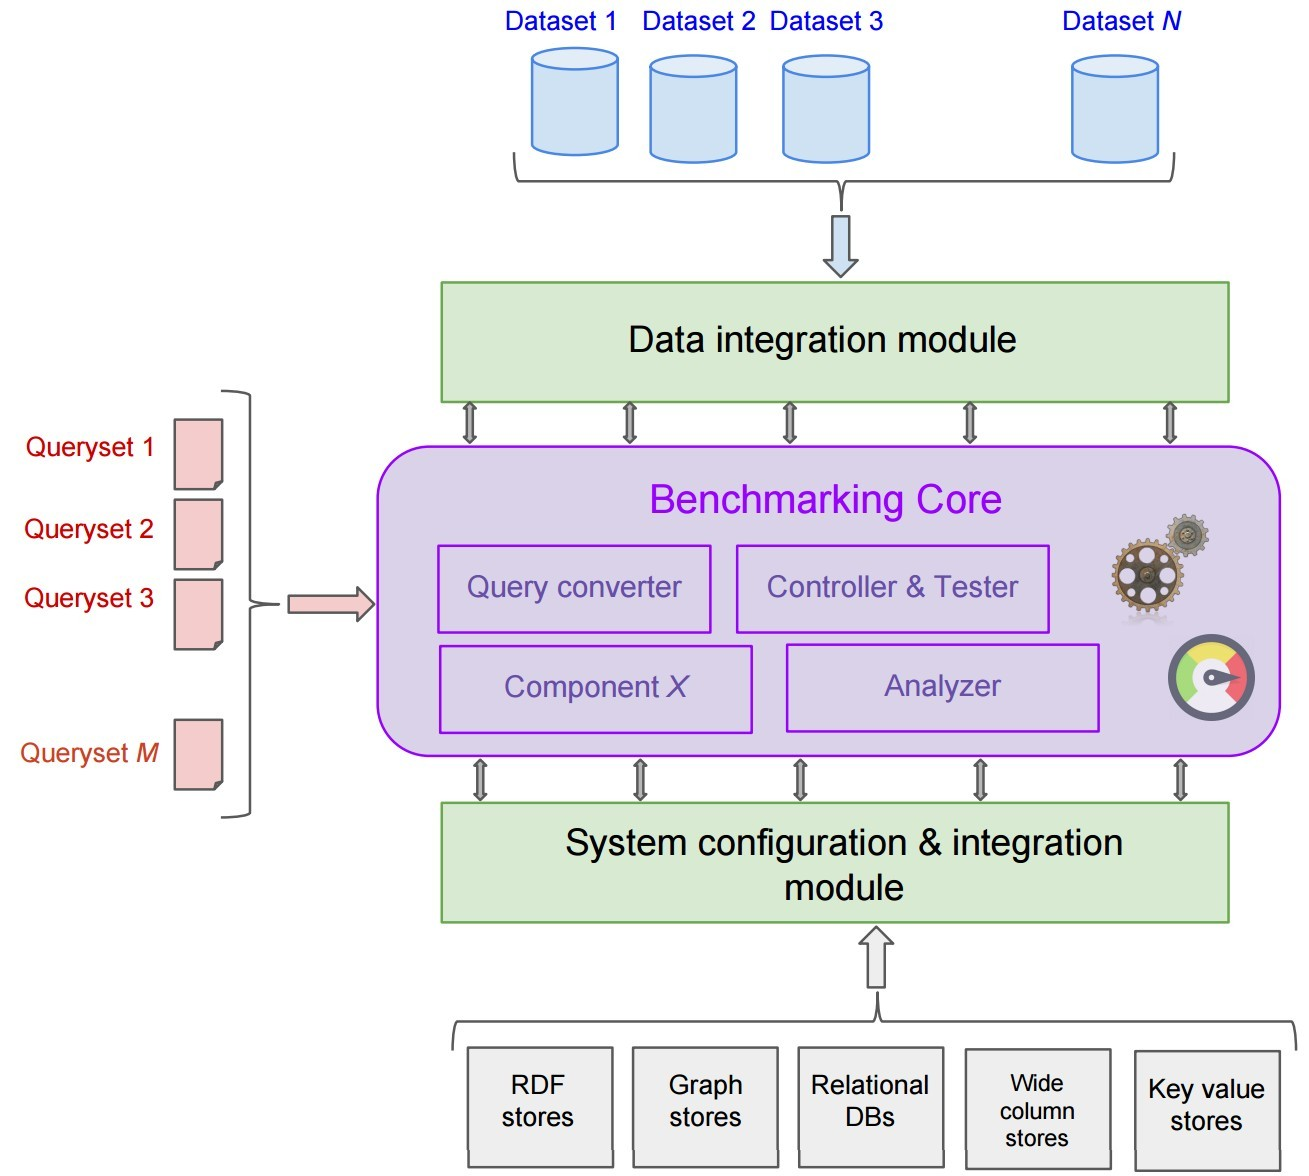
\includegraphics[width=\textwidth]{images/benchmark_arch_new}
            \caption{Architecture of the proposed benchmarking framework.}
            \label{fig:benchmark_arch}
        \end{figure}
    
    \subsection{Challenges}
    \todoinline{pending}
        \begin{enumerate}
            \item Challenge 1 \framebox[1.03\width]{C1}: Normalising the data
            Define the problem, possibly with a simple diagram and/or a table of different data formats which are required by these tools.
            \item Challenge 2 \framebox[1.03\width]{C2}: Converting the Queries
            Define the problem of query conversion and why it is needed to be solved. Again with a block diagram from the framework and/or a table displaying the discrete needs of each tool in terms of query languages they use.
            Also raise the issue of lack of a standard/intermediate representation mechanism. Why it is needed so badly, now more than ever.
            also propose a solution approach in the block diagram (as mentioned above).
            \item Challenge 3 \framebox[1.03\width]{C3}: Performance features/indicators: what features, metrics, indicators to consider for the eval apart from the ones that exist such precision recall, index, storage, graph algos, etc.
        \end{enumerate}
        
    \subsection{Research gaps to be filled by LITMUS}
    \todoiteminlinedone{Harsh}{all}{Please review}
    The artifacts produced by the research and development activity to be undertaken for the LITMUS project can be grouped in to two groups: \textit{(A1)} scientific studies/surveys and \textit{(A2)} software deliverables. 
    
    \framebox[1.03\width]{A1}\textit{ Scientific studies/surveys such as:} 
        \begin{itemize}
            \item Survey of the query language expressivity features for overcoming the language barrier
            \item A study of a wide range of indexing and storage techniques used for fast and efficient retrieval of structured data
            \item A detailed study of performance features/indicators in the domain of query and data over RDF (structured) data. On top of the existing performance evaluation measures, we will study and analyse a series of other features such as the design of indexes and corresponding data structures on the retrieval performance for structured data. A detailed examination of the correlation between query typology and data storage and retrieval mechanisms.
        \end{itemize}
        
        \framebox[1.03\width]{A2} \textit{software deliverables (i.e. algorithm(s), tools, etc) including:} 
        \begin{itemize}
            \item A mechanism/range of solutions for converting RDF data to multiple data formats, such as: CSV (Comma Separared Value), JSON (JavaScript Object Notation),  and SQL (Structured Query Language) for ensure easy data loading for cross domain DMS's. 
            \item A novel SPARQL to any query converting mechanism
            \item A wrapper allowing easy integration and deployment of third party DMS's for realistic benchmarking
            \item A universal benchmarking platform: We will develop an open extensible framework for cross domain performance evaluation of query and storage in RDF DMS's. The proposed benchmark will be scalable for large scale evaluations (such as Big Data).


\section{NoSQL Data management systems}
\todoiteminline{Harsh}{all}{I propose we merge this in the motivation, making it an independent section rather than a subsection. We have to focus on why we are proposing such a framework. Mentioning these diverse systems will only strengthen our claims}

  
    RDF stores
    %\subsubsection{Jena}
    %\subsubsection{Sesame}
    %\subsubsection{4store}
    %\subsubsection{Redland}
    %\subsubsection{Strabon}
    %\subsubsection{BrightstarDB}
    %\subsubsection{\color{red}{system... n}}
    
    Graph stores
    %\subsubsection{Neo4J}
    %\subsubsection{Titan}
    %\subsubsection{Giraph}
    %\subsubsection{InfiniteGraph}
    %\subsubsection{FlockDB}
    %\subsubsection{Sparksee}
    %\subsubsection{\color{blue}{system... m}}
    
    %\subsection{Multi-model stores}
    %\subsubsection{\color{green}{system... o}}
    
    Key-Value stores
    %\subsubsection{K-V store 1}
    %\subsubsection{K-V store 2}
    
    Wide Column stores
    %\subsubsection{W-C store 1}
    %\subsubsection{W-C store... r}
    
    Document-oriented stores
    %\subsubsection{D-O store 1}
    %\subsubsection{D-O store 2}





%========================================EVALUATION======================================
\section{Evaluation parameters}
    \todoiteminline{Harsh}{co-authors}{Since we mentioned that we plan to produce a study of a wide range of performance indicators in sec 3.4, I propose we can just leave this for now with a small summary table of metrics used these days. or we can just skip this section all at once.}
    \subsection{Evaluation parameters}
    System n VS m VS o VS p VS r VS s 
    
    
\section{Case study?, User scenairo?}
\todoinline{do we need one?}


%========================================RELATED WORK======================================
\section{Related work}\label{relwork}
    \todoiteminline{Harsh}{co-authors}{This is pending}
    Nowdays, the most popular model of relational databases have standard banchmark suites such as TPC~\cite{Nambiar2011} benchmark suite. However, the emerging field of Linked Data still lacks such support. We reivew current state-of-the-art work done on Linked Data banchmarking and explain how our aproach will enhances over them.
    

    \begin{itemize}
        \item survey papers and other formal publications on benchmarking different graph stores, comparison of various triple stores and so on
        \href{https://docs.google.com/document/d/1DbtHvE4oaSuusPjeM2nGNBzrRArQt_rlCh3J5g2aIAE/edit?usp=sharing}{Literature review of Related Work}
        
        \item Papers on data, queries and other tools used for benchmarking
    \end{itemize}
    
    
    Other benchmarks, Other such frameworks? \\
    LDBC council work to be cited
    Gerbil to be cited
    BAT-framework ot be cited

    
    

%========================================CONCLUSION AND FUTURE WORK======================================

\section{Conclusion \& Future directions}
We plan to do what we said in the order we said!
\section*{Acknowledgments}\label{sec:Acknowledgments}
This project is supported by funding received from the European Unions Horizon 2020 research and innovation program under the Marie Sklodowska-Curie grant agreement No 642795 (WDAqua ITN).

\bibliographystyle{abbrv}
\bibliography{ref}

\end{document}